\chapter{Introducción}

Los enlaces de hidrógeno (EH) son de las interacciones no covalentes más
importantes dentro de la química, por lo que en esta tesis se plantea el
problema de cómo la energía de interacción en los EHs, entre moléculas de agua,
pude verse afectada dependiendo de la conectividad de éstas moléculas. Para
resolver este problema se propone el estudio de cúmulos de agua de diferentes
tamaños y con diferentes tipos de coordinación.  Para llevar acabo este estudio
se utilizó la partición de la energía electrónica de átomos cuánticos
interactuantes (IQA por sus siglas en inglés), metodología que permite calcular
la energía de interacción entre moléculas dentro de un cúmulo molecular. Se
clasificaron las moléculas dentro de los cúmulos de agua de acuerdo con su
conectividad y, de este modo, extender el trabajo realizado con anterioridad
sobre la fortaleza jerárquica de los EHs en función de la conectividad de las
moléculas presentes en la interacción (\textit{Phys. Chem. Chem. Phys.}, 2016,
\textbf{18}, 19557-19566), incluyendo ahora, moléculas de agua
tetracoordinadas.

Los resultados muestran que las energías de formación de los EHs entre
moléculas tetracoordinadas son similares, pero menores, que las encontradas en
el caso tricoordinado. No obstante, la tetracoordinación es preferida por $i$)
fortalecer los EHs asociados a la aparición de moléculas de H$_2$O dobles
donadoras de H y dobles aceptores, además de $ii$) la aparición de un mayor
número de interacciones favorables para el sistema. Además se encontró que los
EHs más fuertes y débiles están en los casos de tricoordinación, mientras que
las interacciones entre moléculas tetracoordinadas se encuentran a la mitad de
la escala.

En general se espera que los resultados obtenidos en esta tesis proporcionen
ideas importantes sobre las interacciones presentes dentro de los cúmulos de
agua, en especial en aquellas presentes entre moléculas de agua tri- y
tetracoordinadas. Asimismo, esperamos que nuestras conclusiones ayuden en el
entendimiento de las interacciones y fenómenos al rededor del hielo
$\mathrm{I_{h}}$.

\section{El Agua}

El la antigüedad, el agua era considerada como un elemento, no fue hasta 1781
que, Henry Cavendish (1731-1810), postula que el agua es una combinación de
substancias más simples~\cite{sanchez2006revolucion}. Hoy en día es posible
describir a la molécula de agua como la unión entre un átomo de oxígeno y dos
de hidrógeno por medio de enlaces simples, además el átomo de oxígeno posee dos
pares de electrones libres que le confieren propiedades características al
agua~\cite{biology}. La primera demostración de que el agua estaba compuesta
por dos volúmenes de hidrógeno por cada uno de oxígeno fue propuesta por
Gay-Lussac y von Humboldt en 1804. 

\subsection{Propiedades del agua}

A continuación, se enlistan algunas de las propiedades físicas y químicas
que hacen del agua una de las substancias más importantes para la
vida en la Tierra.

\begin{itemize}

\item Presenta un equilibrio de autoprotólisis en la que una molécula acepta
un protón para formar un ion hidronio y la molécula que dona el protón se
transforma en un ion hidroxilo~\cite{mcmurry}.
\item La movilidad iónica del ion hidronio, en solución acuosa, es
inusualmente alta debido a su particular mecanismo de migración~\cite{voet}.
\pagebreak
\item Es translúcida en la porción visible del espectro
electromagnético, con un color azul~\cite{Braun1993}. Por ello
las plantas pueden llevar a cabo la
fotosíntesis, cuando se encuentran sumergidas en agua.
\item El valor de la entalpía de fusión del agua es inusualmente grade,
\SI{333.6}{\joule \per \gram} a \SI{0}{\celsius}~\cite{noauthororeditor2007handbook}.
\item Posee un alto valor de tensión superficial (\SI{72.88}{\milli
\newton \per \meter} a \SI{20}{\celsius}) debido a la fuerte cohesión de sus
moléculas~\cite{dean92:LHC}.
\item Posee altos puntos de fusión y ebullición para ser una molécula
de bajo peso molecular~\cite{morrison}.
\item Es considerada el mejor regulador térmico de la Tierra debido a su alto
calor específico (\SI{4.184}{\joule \per \kelvin \per \mole}), por ejemplo el del hierro es
de \SI{0.8}{\joule \per \kelvin \per \mole}~\cite{resnick}.
\item Alcanza su máxima densidad volumétrica de masa en forma líquida
(\SI{999.9749}{\kilo\gram\per\cubic\meter}) a \SI{4}{\celsius}~\cite{Tanaka_2001}.
\item Tiene un cambio de volumen de fusión negativo, por lo que la densidad
del estado líquido es mayor que la del estado sólido~\cite{serway2001fisica}.
\item Es un buen aislante eléctrico. Sin embargo, ante la presencia de iones
se convierte en un conductor de corriente eléctrica~\cite{chang}.
\end{itemize}

\subsection{Usos del agua}

Debido a su gran abundancia en el planeta, además de ser fundamental para la
vida como la conocemos, el agua ha sido protagonista de diversos estudios en
varias ramas de la ciencia. Actualmente la contaminación del agua, en especial
la de consumo humano, es un tema que ocupa a gran parte de la comunidad
científica debido al gran riesgo que representa el consumo de ciertos
contaminantes~\cite{Pandey2014, Bove1995}.

\subsubsection{Agua en la biología}

El agua comprende aproximadamente el 80 \% de la masa de las células vivas. El
estudio de las propiedades del agua intracelular se torna difícil debido a que
no es posible aplicar algunos métodos fisicoquímicos al interior de la célula.
Por otra parte, el carácter multicomponente del estudio, debido al gran número
de interacciones, ya sean intra o extracelular, del agua, resulta en una gran
variedad de conclusiones acerca de las propiedades del agua
intracelular~\cite{Cooke1974}.

Este tipo de estudios ha dado paso a una controversia entre quienes consideran
que la mayor parte del agua dentro de las células tiene propiedades similares a
las del líquido normal y quienes consideran esencialmente que toda el agua
intracelular es ``bound water''~\cite{BenNaim1992, Hepler1969}. Esta ``bound
water'' refiere a las moléculas de agua altamente ligadas a la superficie de
las proteínas, por lo que estas moléculas de agua no poseen, en términos
prácticos, movilidad rotacional ni traslacional~\cite{Bagchi}. Estas opiniones
divergentes conducen a predicciones muy diferentes para muchos aspectos dentro
de la biología celular.


\subsubsection{Observatorio de rayos gamma HAWC}

Uno de los usos más actuales que se tiene para el agua es el de observar la
Radiación Cherenkov. El estudio de esta radiación de manera rigurosa fue
realizado por Pável Cherenkov~\cite{cherenkov}, trabajo por el cual se le
otorgó el Premio Nobel de Física en 1958. Su fenomenología es similar a la que
se tiene cuando un objeto supera la velocidad del sonido en su medio de
propagación. La radiación de Cherenkov es una onda de choque, entre las ondas
electromagnéticas, con un singular brillo de tono azulado en agua; observable,
por ejemplo, en reactores nucleares.

El observatorio de rayos gamma HAWC que se encuentra en el flanco norte del
volcán Sierra Negra, en el estado de Puebla, fue diseñado para la detección de
rayos gamma de origen cósmico (con energías entre \SI{100}{\giga \electronvolt}
y \SI{100}{\tera \electronvolt})~\cite{HAWC}, a través la medición de
partículas producto de una cascada atmosférica. 

Una cascada atmosférica es un proceso cuántico de alta energía que se
desarrolla en la atmósfera terrestre cuando un rayo de alta energía (cósmico,
gamma o primario), penetra la atmósfera. Esta colisión inicial produce una
reacción en cadena que se observa como una cascada de partículas viajando a
velocidades cercanas a la de la luz. Existiendo dos tipos: $i$) las cascadas
electromagnéticas y $ii$) las cascadas hadrónicas~\cite{rao1998extensive}. La
primera produce, a través de una interacción con el campo eléctrico de los
átomos de la atmósfera, un par electrón-positrón que, a su vez, producen otros
rayos gamma encadenadamente hasta que la energía baja a menos de
\SI{80}{\mega\electronvolt}, donde ya se producen otros fenómenos tales como el
efecto Compton y absorción fotoeléctrica.  En el segundo tipo de cascada
atmosférica, la partícula de alta energía interactúa directamente con el núcleo
de un átomo, produciendo varios iones y partículas elementales, como los piones
($\pi^0$, $\pi^+$, $\pi^-$), y debido a que los $\pi^0$ decaen rápidamente a
dos rayos gamma, producen nuevas interacciones para el efecto de cascada.

El uso del agua es fundamental para la detección en este observatorio, debido a
que el HAWC está compuesto por \num{300} detectores de radiación Cherenkov en
agua, donde cada detector tiene un tanque de \SI{7}{\meter} de diámetro y
\SI{5}{\meter} de alto, como se observa en la Figura \ref{dino_cherenkov}, en
los cuales se almacenan \SI{180000}{\liter} de agua ultra pura.  En la base de
estos contenedores hay tubos fotomultiplicadores, para así detectar la luz
tenue resultante de la radiación Cherenkov.

\begin{figure}
    \centering
    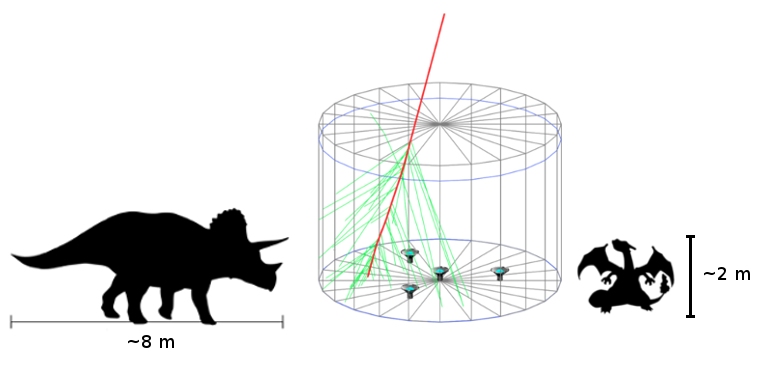
\includegraphics[width=0.80\textwidth]{2/img/dino_cherenkov}
    \caption{Comparación de tamaños de los tanques de agua del HAWC con un triceratops
(dinosaurio de finales del Cretácico) y Charizar (pokémon).}
\label{dino_cherenkov}
\end{figure}

\subsubsection{Desintegración del Protón}

Dentro del Modelo Estándar de la Física de Partículas, los protones son
teóricamente estables, debido a la conservación del número
bariónico~\cite{standarmodel}. No obstante, existen hipótesis en algunas
teorías de campo unificado que rompen explícitamente la simetría del número
bariónico, permitiendo el decaimiento del protón en partículas cargadas más
ligeras~\cite{Kuhne:2011zz}.

Observatorios como el Super-Kamiokande tienen como objetivo buscar evidencia
experimental del decaimiento del protón, a través de radiación Cherenkov, que
se produciría tras el decaimiento de algún protón en sus  \SI{50}{\kilo\tonne}
de agua ultra pura, donde la radiación podrá ser observada mediante \num{13}
mil tubos fotomultiplicadores~\cite{Kamioka}.  A lo largo del tiempo que este
observatorio ha estado trabajando no ha detectado aún el decaimiento de algún
protón, pero sí ha dado grandes contribuciones, como la fuerte evidencia de la
oscilación del neutrino, resultado consistente con la teoría de que los
neutrinos tienen masa no nula~\cite{10.2307/26058368}, ésta aportación le
otorgó el Premio Nobel de Física en 2015 a Takaaki Kajita y Arthur B. McDonald.

\subsubsection{Agua en procesos industriales}

Además de los usos antes mencionados, es importante resaltar el uso del agua en
diversos procesos industriales, tales como el de la fabricación de la cerveza.
Debido a la gran necesidad de agua, cerca de \SI{1.2}{\liter} de agua por
botella de cerveza~\cite{grupomodelo}, plantas como la de Zacatecas de Grupo
Modelo, se encuentra justo encima de ocho pozos de agua, con profundidades que
van desde los \SI{150}{\metre} hasta los \SI{500}{\metre}.

Otras industrias en las que el agua es sumamente importante son:

\begin{itemize}
\item Plantas de producción eléctrica
\item Industria textil
\item Industria cárnica
\item Industria minera
\item Industria agropecuaria
\end{itemize}


\subsection{Hielo}

Se suele referir al agua en estado sólido como hielo, aunque existen varios
tipos de arreglos estructurales para el agua en estado sólido, como se muestra
en el diagrama de fases ilustrado en la Figura \ref{diagrama_fases}, el más
común en la vida diaria es el conocido como hielo $\mathrm{I_{h}}$. El hielo
$\mathrm{I_{h}}$ se puede encontrar con facilidad en forma de nieve, escarcha,
granizo o icebergs.  No se debe confundir este término con el de ``hielo
seco'', el cual hace referencia al estado sólido del dióxido de carbono.

\begin{wrapfigure}[13]{r}{0.33\textwidth} %this figure will be at the r
    \centering
    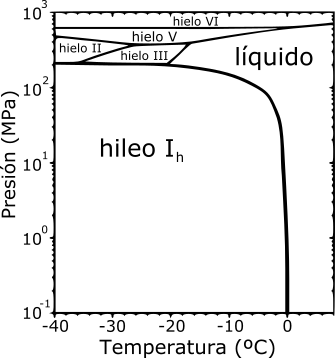
\includegraphics[width=0.31\textwidth]{2/img/Phase_diagram_of_water_}
    \caption{Diagrama de fases del agua, con cuatro de sus posibles arreglos en estado sólido y
    el estado líquido.}
    \label{diagrama_fases}
\end{wrapfigure}
%
El hielo $\mathrm{I_{h}}$ es un modo habitual en el que se puede encontrar el
agua en la naturaleza, aunque es posible encontrar otras fases del hielo, éstas
se encuentran en menor abundancia y en casos más particulares, el hielo
$\mathrm{I_{c}}$ se puede encontrar en casquetes polares en equilibrio
termodinámico con el hielo $\mathrm{I_{h}}$. Encontrar hielo VII es bastante
más inusual, pero posible, debido a las grandes presiones a las cuales el
diamante es formado, se puede encontrar hielo VII dentro de
diamantes~\cite{Tschauner2018}.  El hielo, debido a que es un sólido estable a
temperatura menores a \SI{0}{\celsius}, es considerado como un mineral dentro
de la mineralogía, y es clasificado como un mineral óxido en el grupo 4, debido
a que normalmente se encuentra con muchas impurezas~\cite{Demirbas2010}.

Es un dicho popular ``no hay dos copos de nieve iguales'', pero, como ya se
mencionó, es común encontrar el hielo $\mathrm{I_{h}}$ en los copos de nieve,
por lo que, a pesar de la gran variedad de arreglos, es posible, aunque muy
poco probable, que haya dos copos de nieve iguales.

La humanidad le ha dado diversos usos al hielo, entre ellos, se encuentran los
fines recreativos, como es el patinaje sobre hielo. Además, el uso de la nieve
ha permeado en la cultura a través de diversos juegos, tales como la guerra de
bolas de nieve o hacer muñecos de nieve. Estos usos recreativos evolucionaron
de tal modo que los Juegos Olímpicos de Invierno cuentan actualmente con 15
deportes~\cite{OInvierno}.

\begin{figure}%[h!]
\centering
\begin{subfigure}[b]{0.27\linewidth}
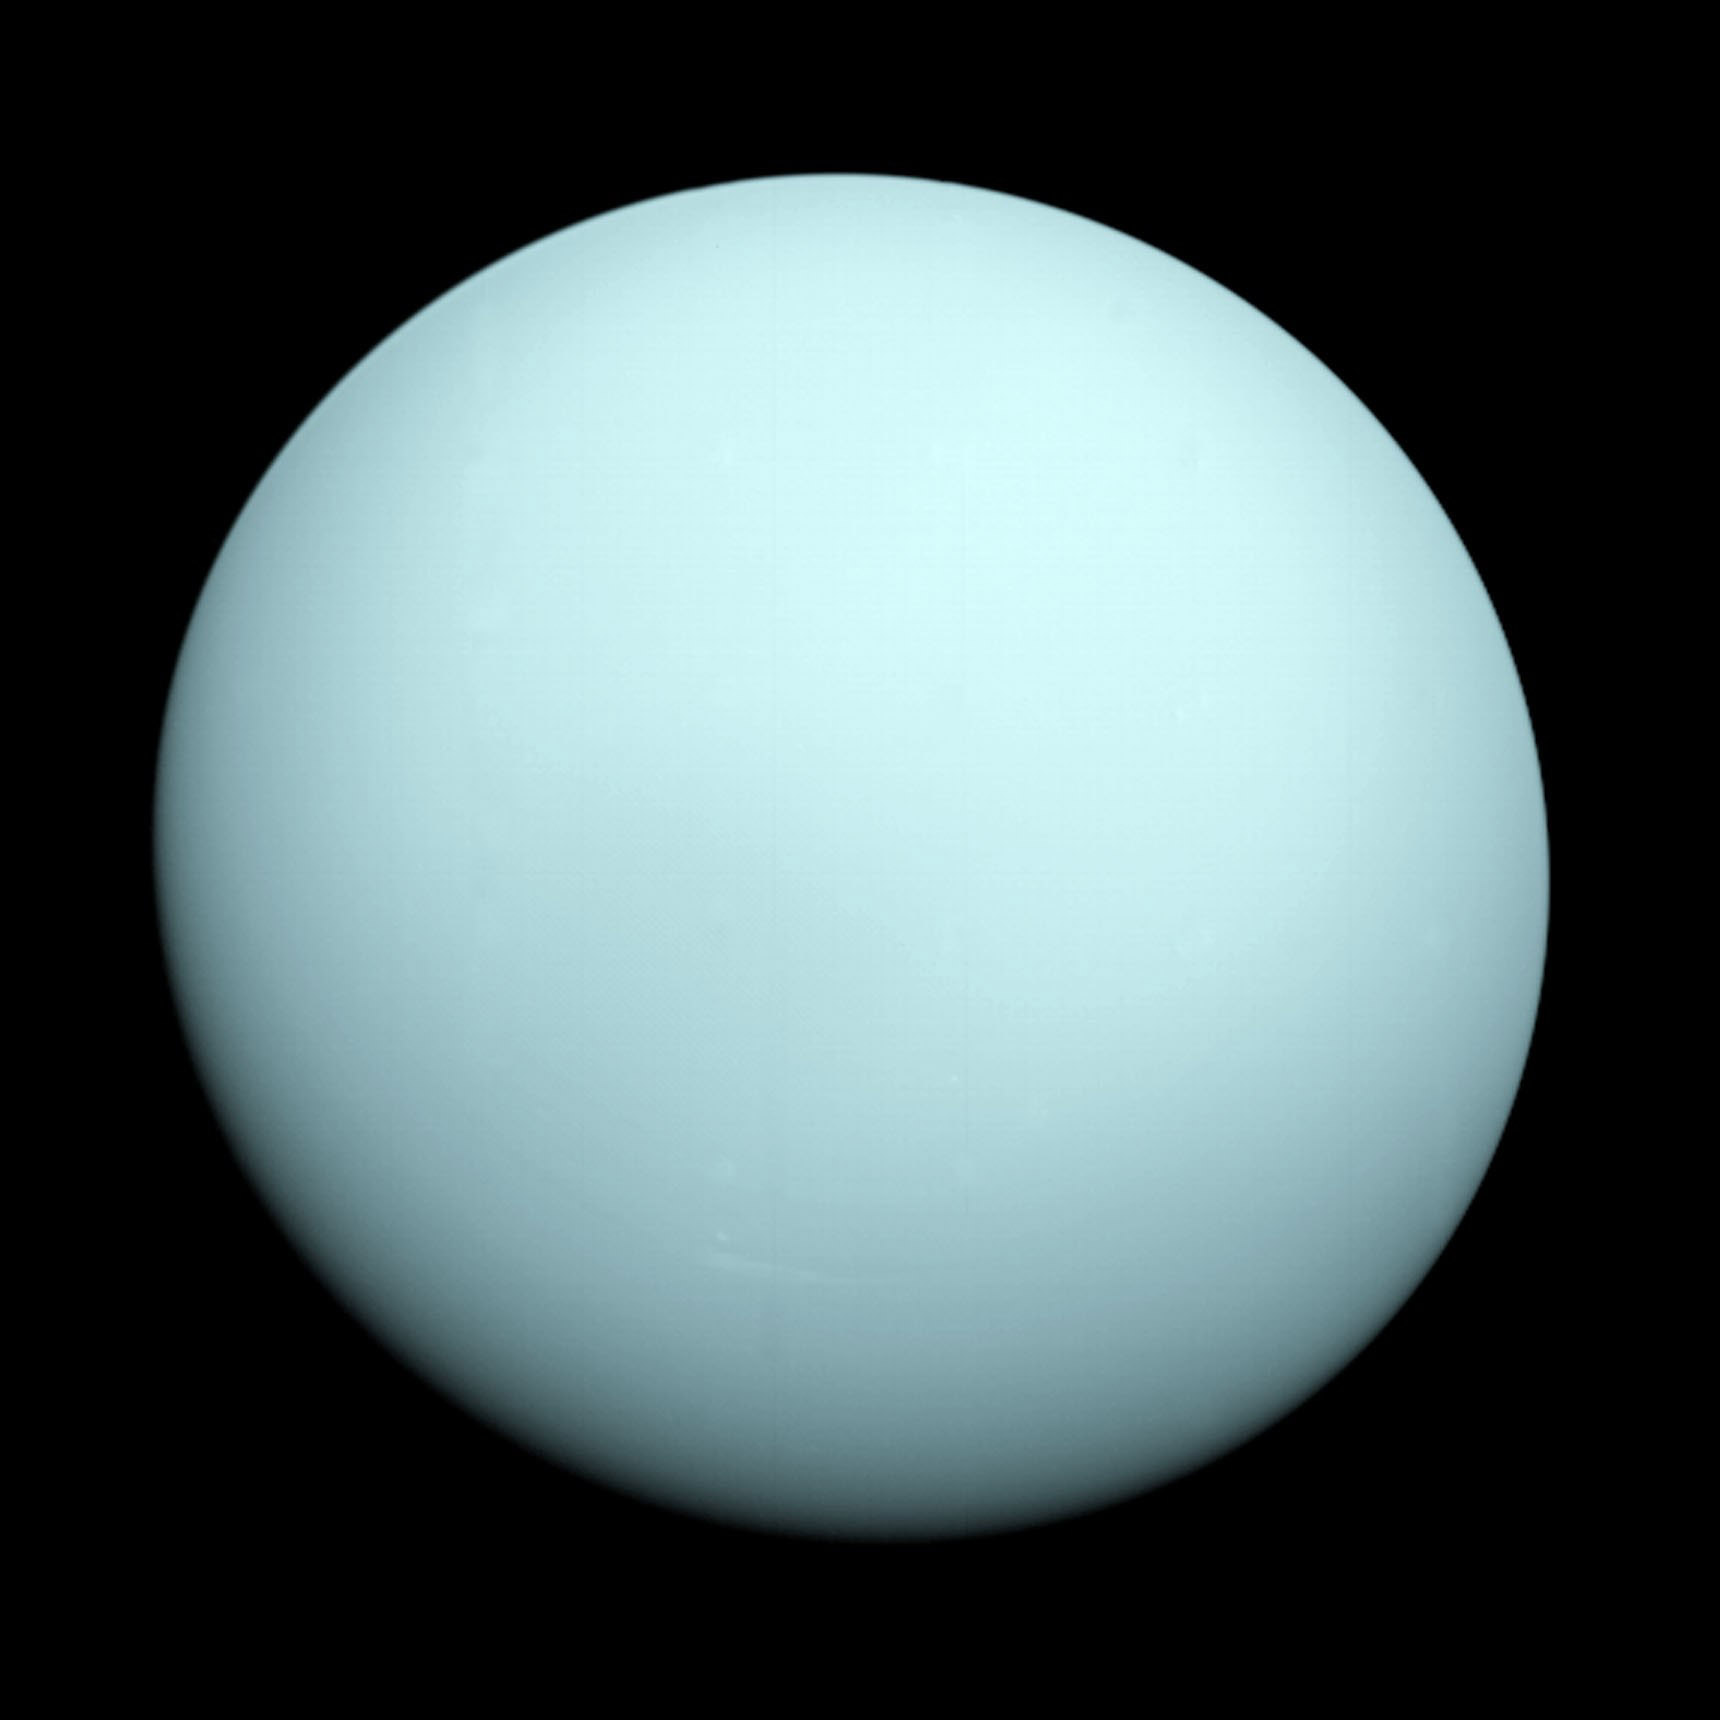
\includegraphics[width=\linewidth]{2/img/imagecuranusvoyager}
\caption{Urano en 1986.}
\label{urano}
\end{subfigure}
\begin{subfigure}[b]{0.27\linewidth}
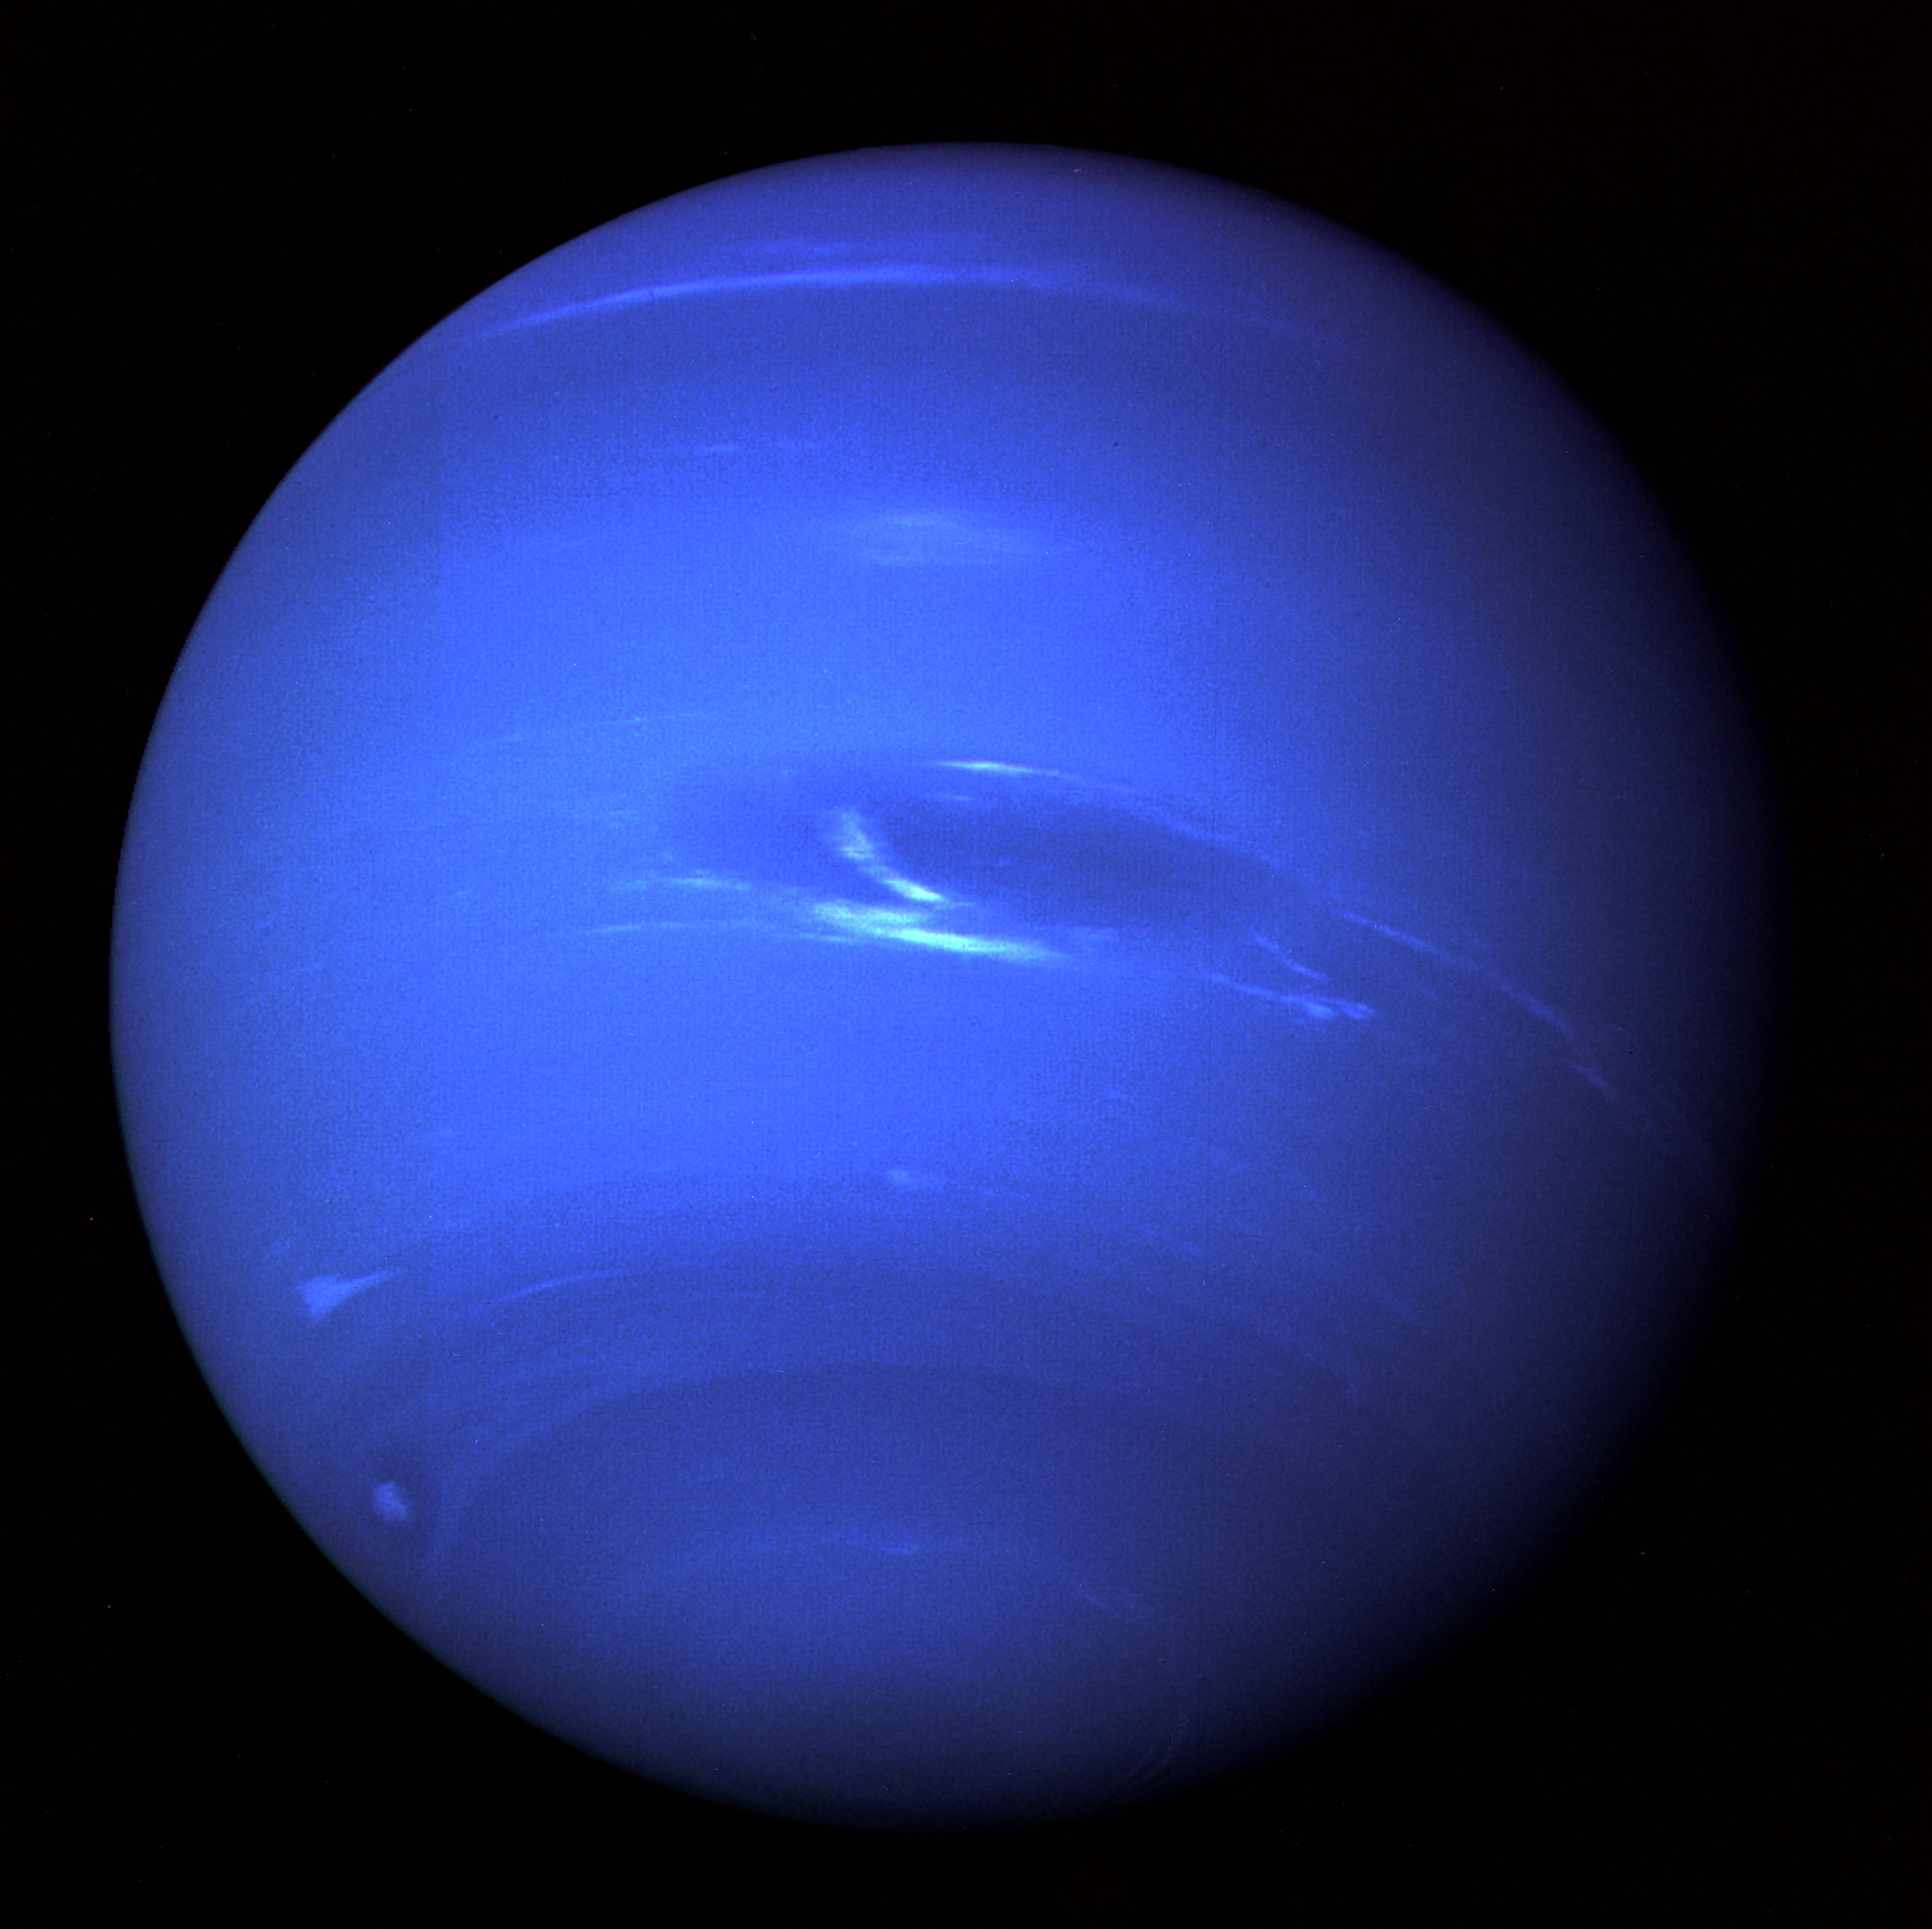
\includegraphics[width=\linewidth]{2/img/imagedneptunevoyager}
\caption{Neptuno en 1989.}
\label{neptuno}
\end{subfigure}
\caption{Fotografías tomadas por la sonda espacial Voyager 2 de la NASA~\cite{urano_neptuno_photo}.}
\label{urano_neptuno}
\end{figure}

El hielo no sólo es abundante en el planeta Tierra, es normal hablar incluso,
dentro de la astronomía planetaria, de los gigantes helados: $i)$ Urano y $ii)$
Neptuno. Este término hace referencia a una subclasificación de los planetas
gigantes, debido a su gran abundancia de hielo, gas y rocas; al contrario de
los otros planetas considerados como gigantes, en los que existe una mayor
cantidad de hidrógeno y helio, por ende llamados gigantes gaseosos. Las
tonalidades característica de Urano y Neptuno se deben a que, dentro de su
composición atmosférica, existe una pequeña cantidad de metano y amoniaco
($\sim$ \num{2} \%) que, junto con el hielo le dan sus particulares tonos a
estos planetas~\cite{Atmospheres_ice}. A través del mismo fenómeno que sufre el
agua en los océanos de la Tierra, son necesarias grandes cantidades de hielo,
metano y amoniaco para que los tonos azules y verdes sean apreciables, como se
muestra en las fotografías (Figura \ref{urano_neptuno}).

\section{Enlace de Hidrógeno}

Las propiedades antes mencionadas del agua son explicadas, en su mayoría, por
un tipo especial de interacción no covalente, el Enlace de Hidrógeno (EH). En
la Figura \ref{4_h2o} se presenta a un grupo de 5 moléculas de agua
interactuando a través de EHs.  El número total de interacciones de EH para
cúmulos grandes, tan grandes como $N_A$, es de $2N_A$. Este entramado de EHs es
lo que provoca que en un sistema exista una cohesión poco usual entre este tipo
de moléculas~\cite{smith2005}.

\begin{wrapfigure}[16]{r}{0.41\textwidth} %this figure will be at the right
    \centering
    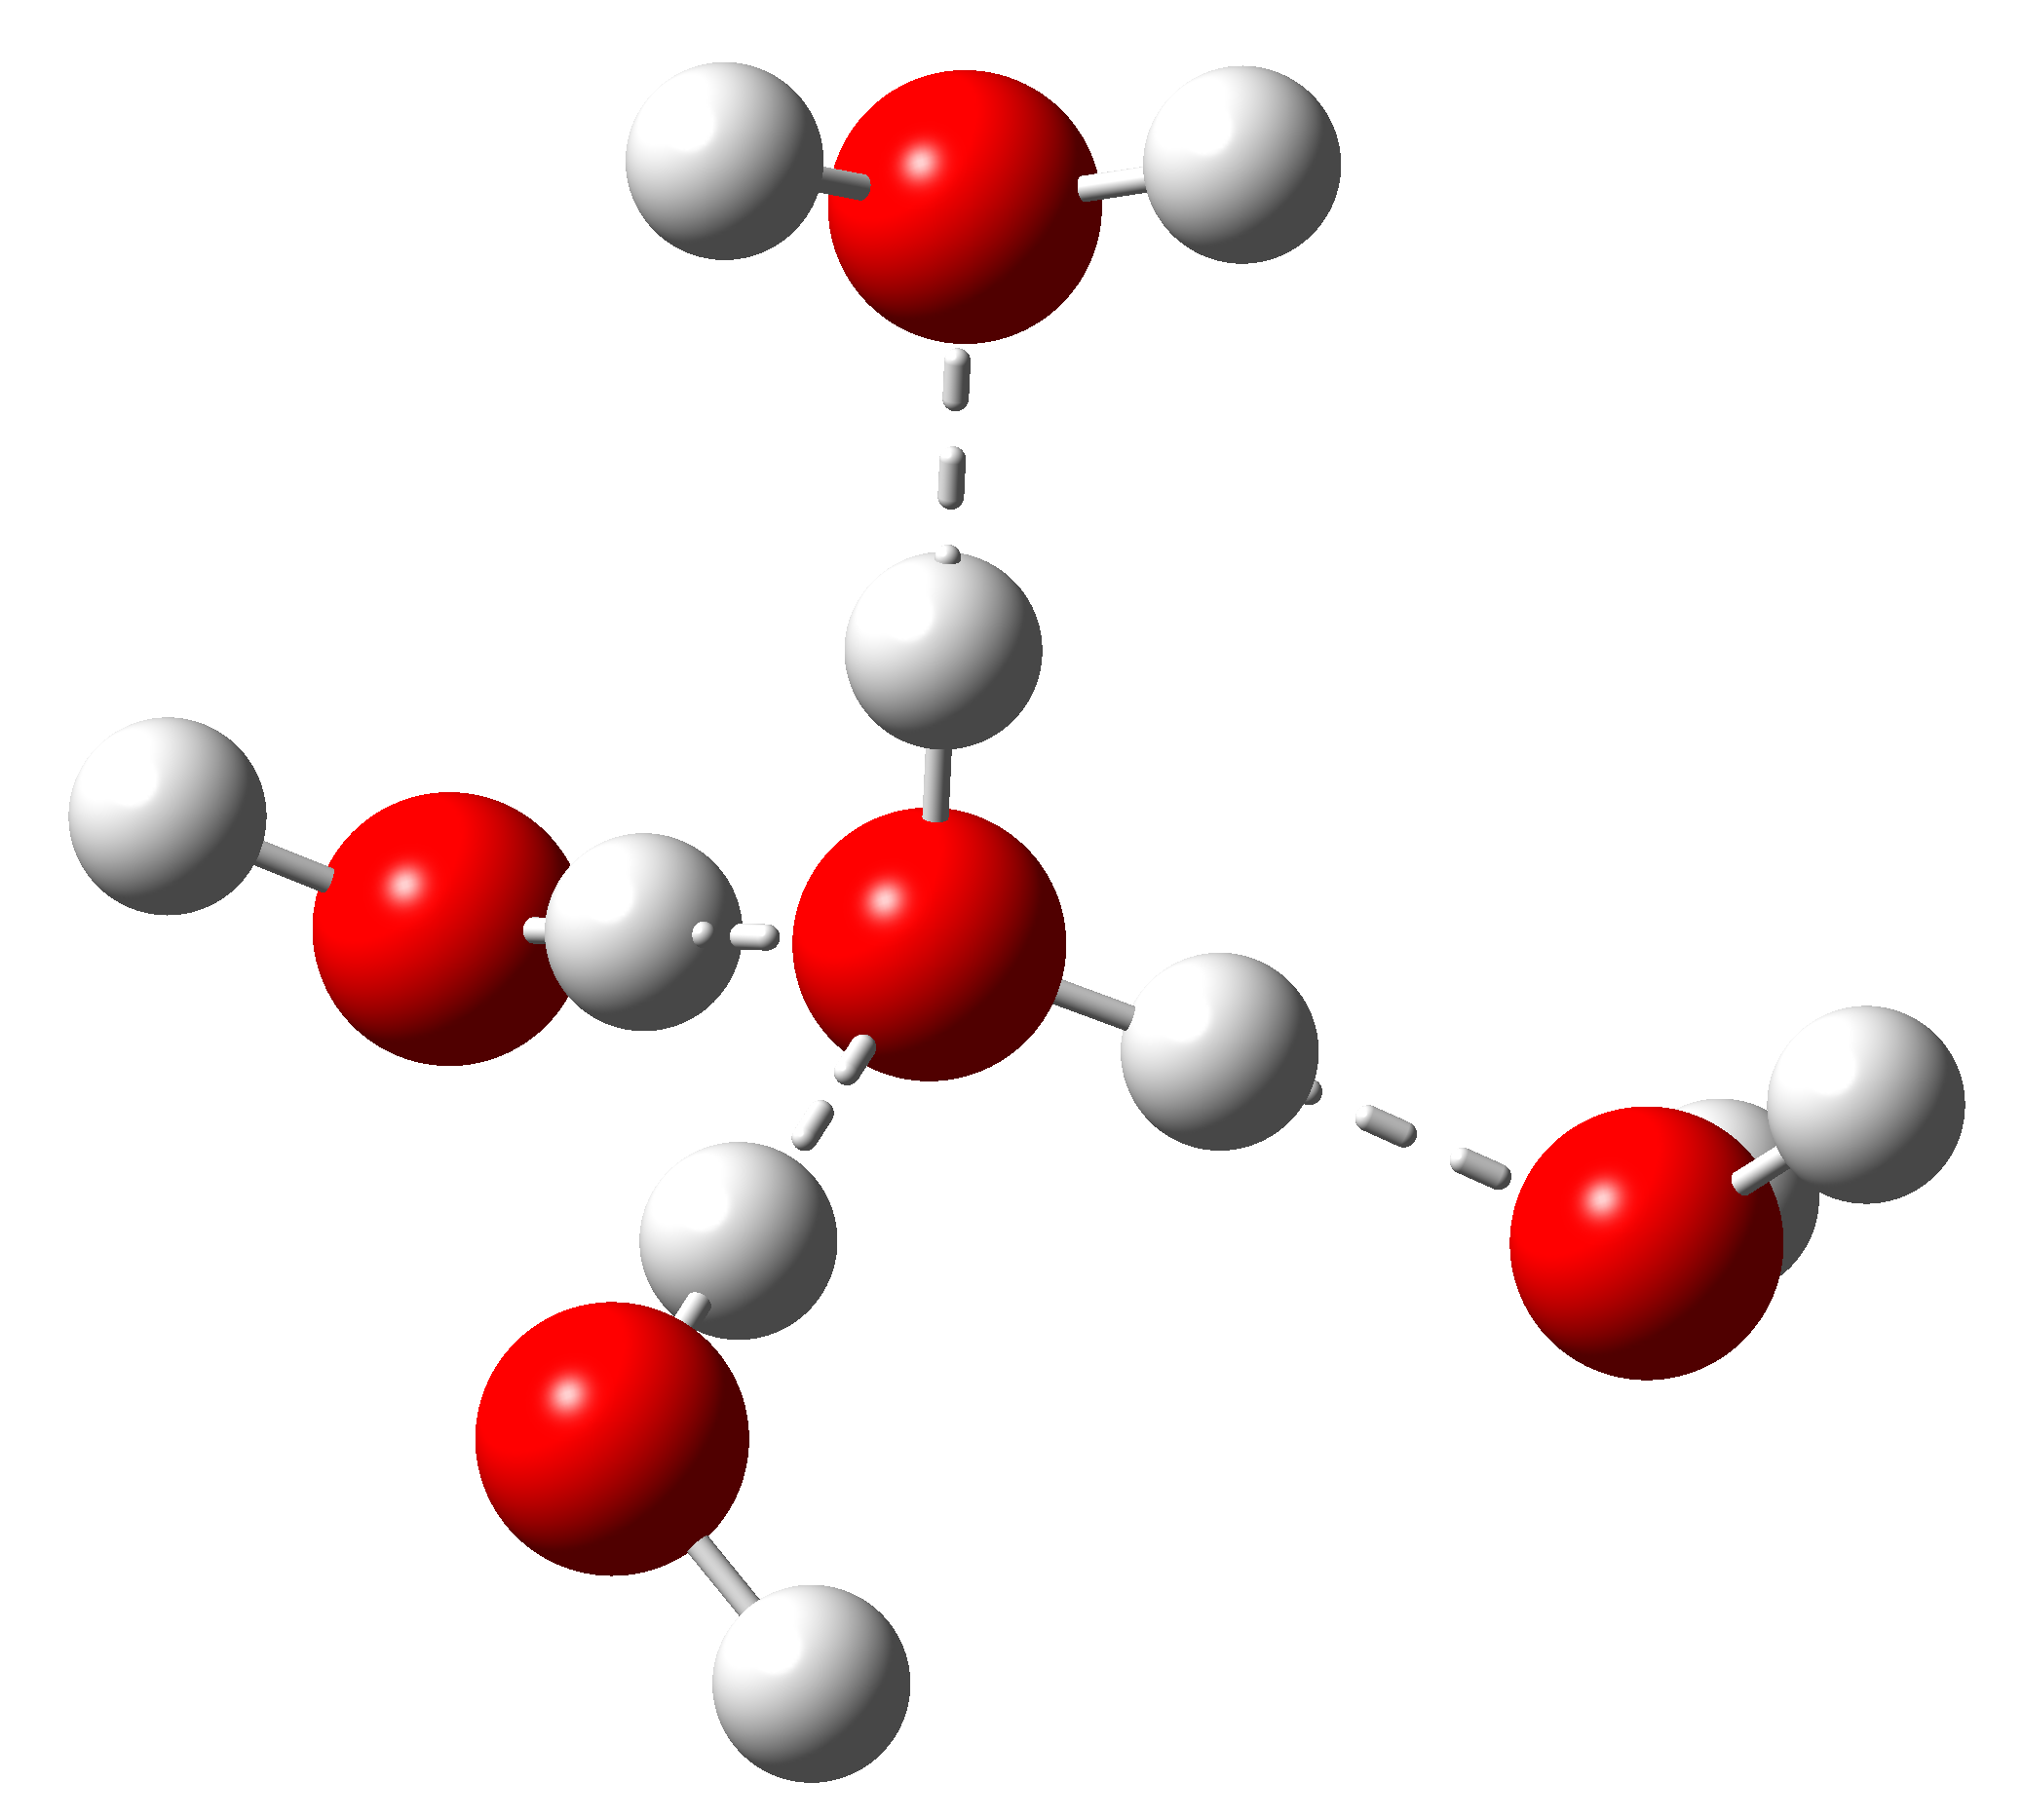
\includegraphics[width=0.41\textwidth]{2/img/4h2o}
    \caption{La molécula de agua central está aceptando dos átomos de hidrógeno y donando
otros dos, por lo que es posible decir que forma 4 EH, en dos toma el papel de
donadora y en los otros dos de aceptora.}
    \label{4_h2o}
\end{wrapfigure}

El EH fue descubierto hace más de cien años y no es posible atribuir éste
hallazgo a un solo autor, tampoco existe una publicación la cual pueda ser
considerada como la iniciadora de éste término. Publicaciones especializas en
esta interacción comenzaron a aparecer a finales del siglo XIX, en especial
dentro de la literatura inglesa y alemana, sin embargo la relevancia del EH aún
no era reconocida~\cite{steiner}. Estudios más detallados, conceptos más claros
y específicos fueron desarrollados a partir de 1920~\cite{steiner}. El primero
en utilizar el término enlace de hidrógeno fue Pauling en 1931~\cite{gilli}.  A
finales de la década de 1930, se estableció una explicación del EH, y éste se
describía como un fenómeno puramente clásico en términos electrostáticos,
debido a que en su mayoría, los ejemplos encontrados eran de interacciones
débiles.  Actualmente esta idea ha sido sustituida debido al elevado número de
ejemplos de EHs con una mayor energía, en donde no es posible despreciar las
contribuciones no clásicas en esta interacción.

El enlace de hidrógeno se encuentra definido por la IUPAC como:

\begin{quote}
El enlace de hidrógeno es una interacción atractiva entre
una molécula o fragmento molecular X-H y un átomo A en la misma u
otra molécula, en la cual X es más electronegativa que H y existe 
evidencia de la formación de un enlace~\cite{iupac}.
\end{quote}

Ésta interacción se clasifica como de mediano alcance debido a que la distancia
es mayor a la de un enlace covalente, además de ser generalmente más débil que
éstas. Pero sin llegar a ser tan distantes o débiles como las fuerzas de Van
der Waals~\cite{chang}.

Otra definición de EH es propuesta por Steiner~\cite{steiner}:

\begin{quote} 
Una interacción X-H$\cdots$A se llamará enlace por puente de
hidrógeno si $i$) constituye un enlace local y $ii$) X-H funge como un
donador de protón hacia A.
\end{quote}

\noindent Esta forma de describir al EH es lo bastante más flexible como para
incluir una amplia gama de fenómenos en los que se involucra una interacción no
covalente con un átomo de hidrógeno. La definición de Steiner es igualmente
válida para los EH más simples, aquellos en los cuales el donador X posee
solamente un hidrógeno capaz de interactuar con un aceptor A que tiene
únicamente un par de electrones disponible para formar el
enlace~\cite{scheiner}, como para interacciones más complejas como los EHs
involucrados en el plegamiento de proteínas.

\begin{figure}[b!]
\centering
\begin{subfigure}[b]{0.3\linewidth}
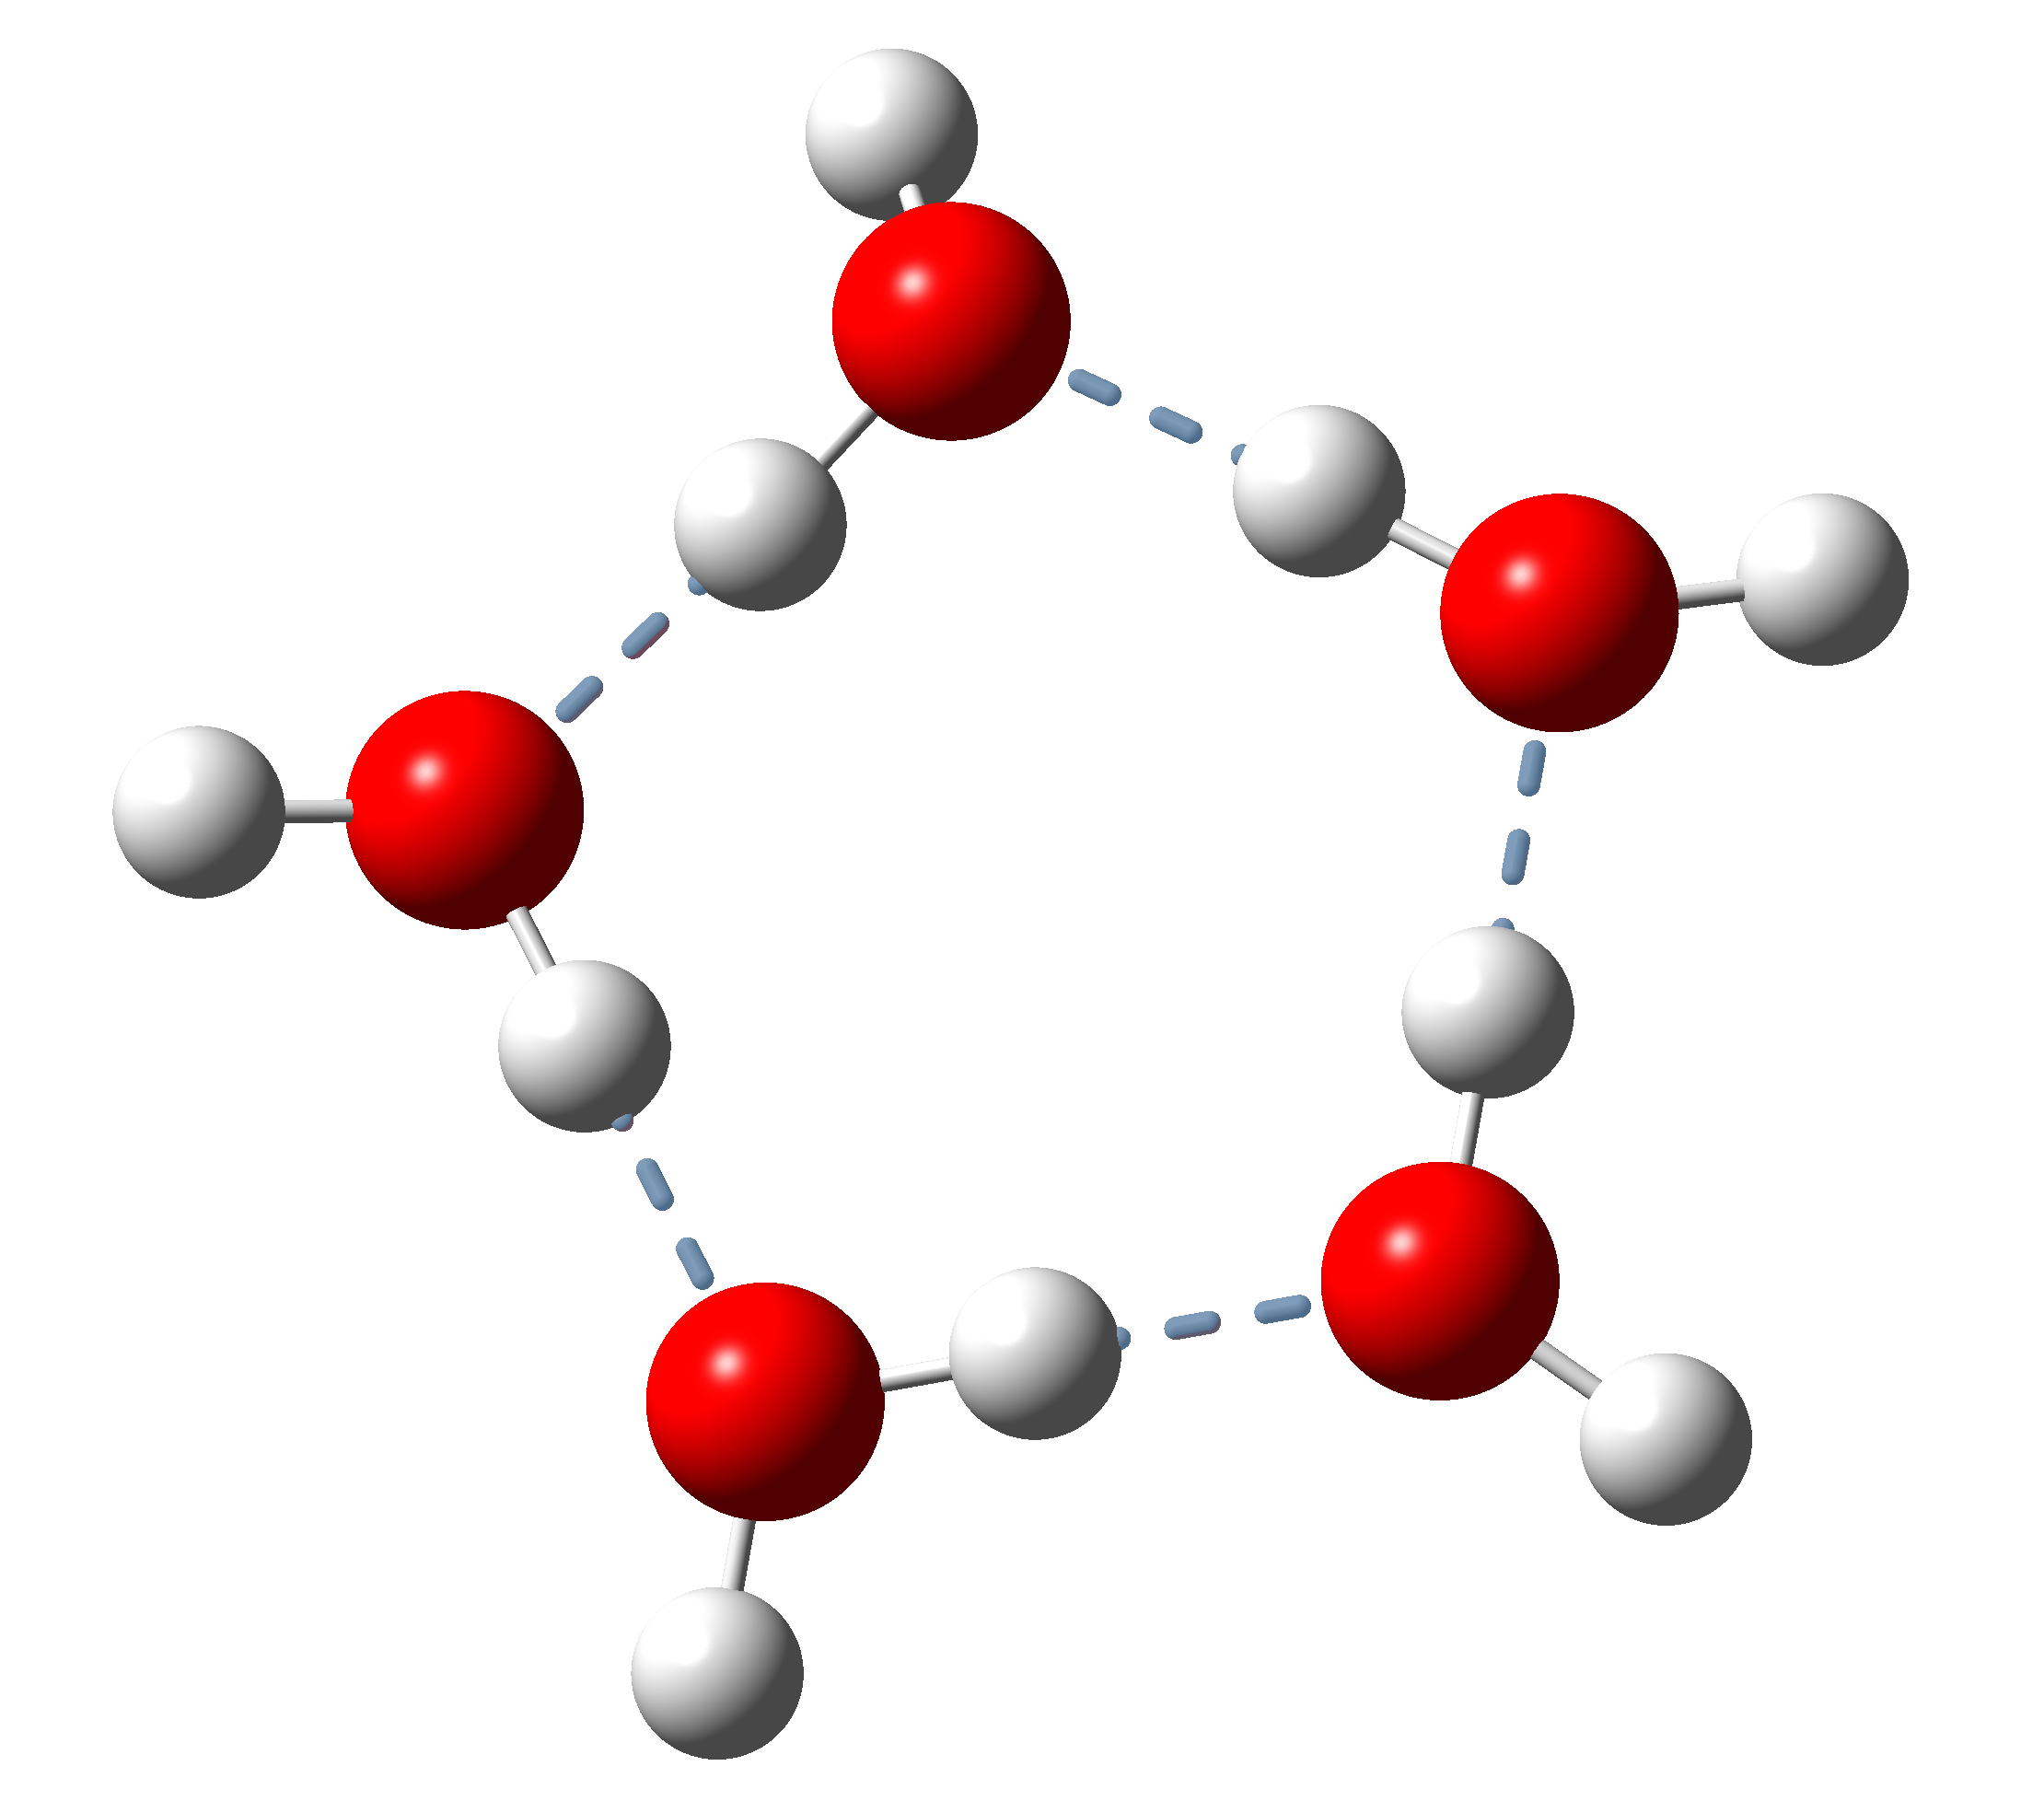
\includegraphics[width=\linewidth]{2/img/pentamero}
\caption{Homodrómico}
\label{pentamero}
\end{subfigure}
\begin{subfigure}[b]{0.3\linewidth}
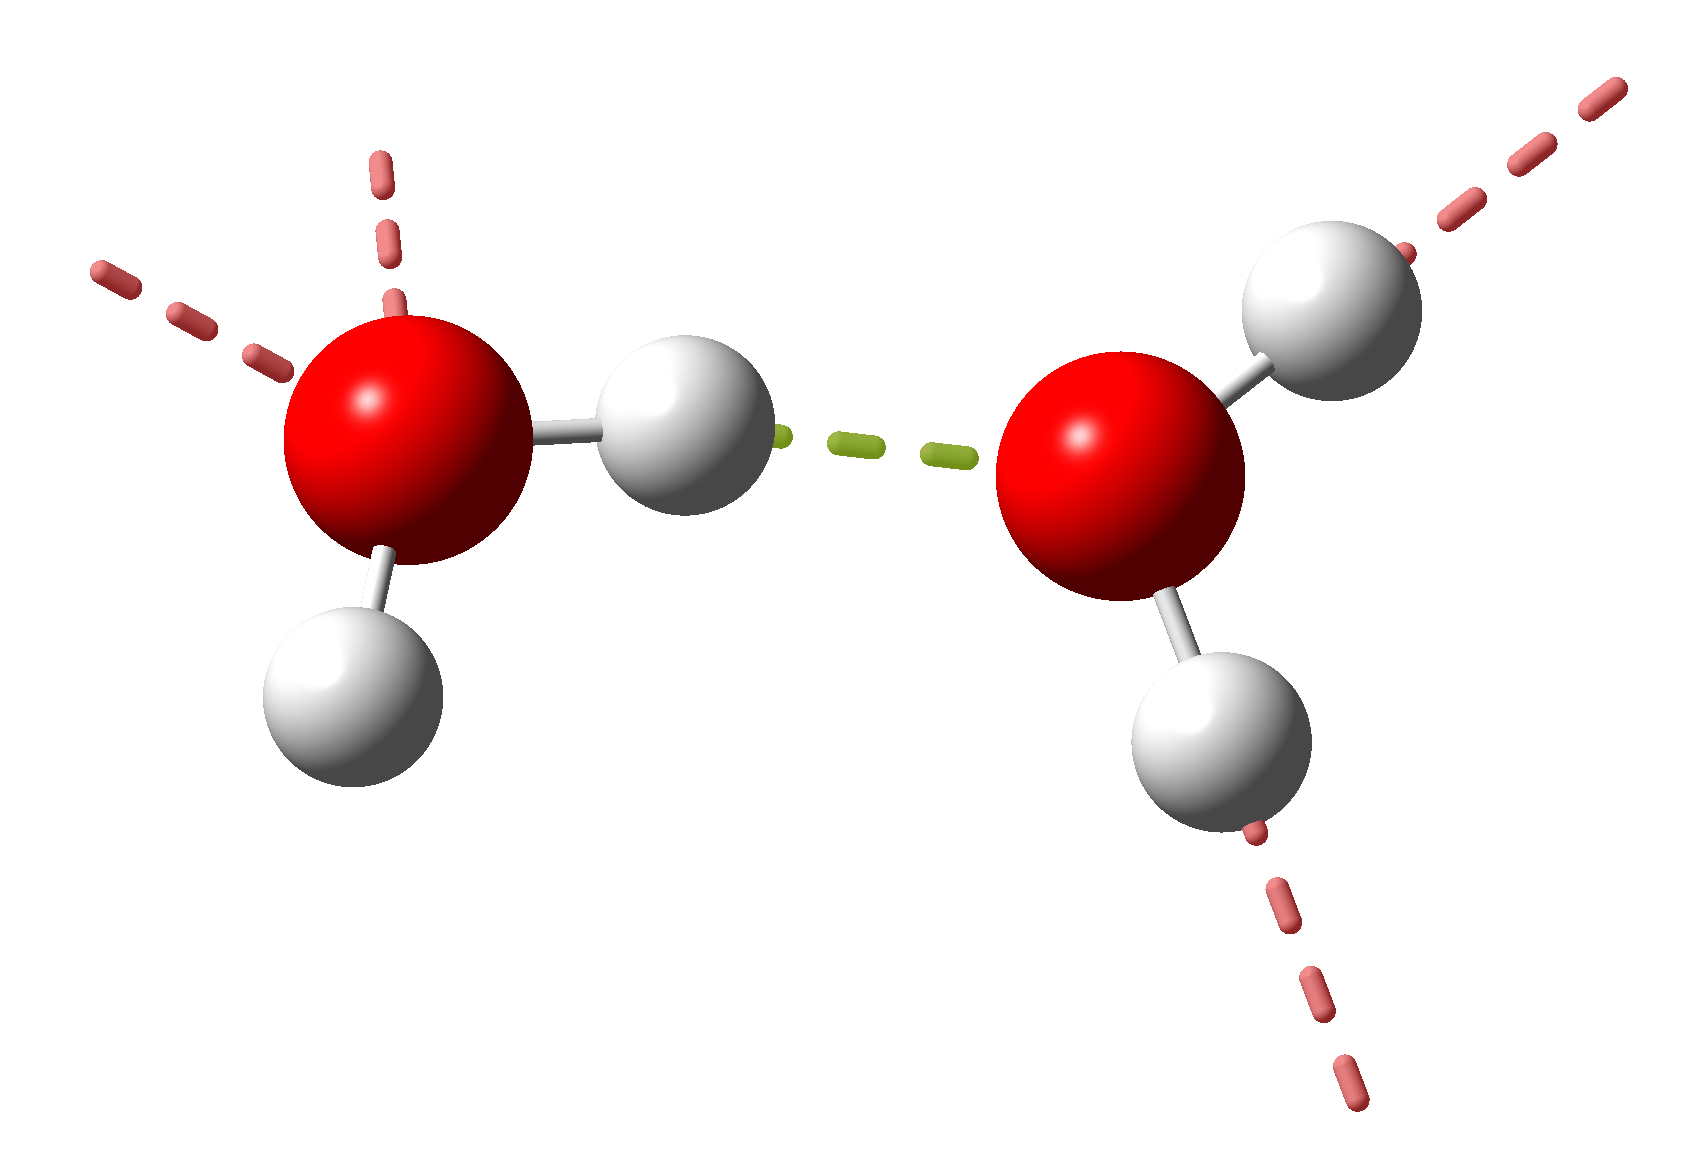
\includegraphics[width=\linewidth]{2/img/dimero_b}
\caption{Cooperativo}
\label{dimero_b}
\end{subfigure}
\begin{subfigure}[b]{0.3\linewidth}
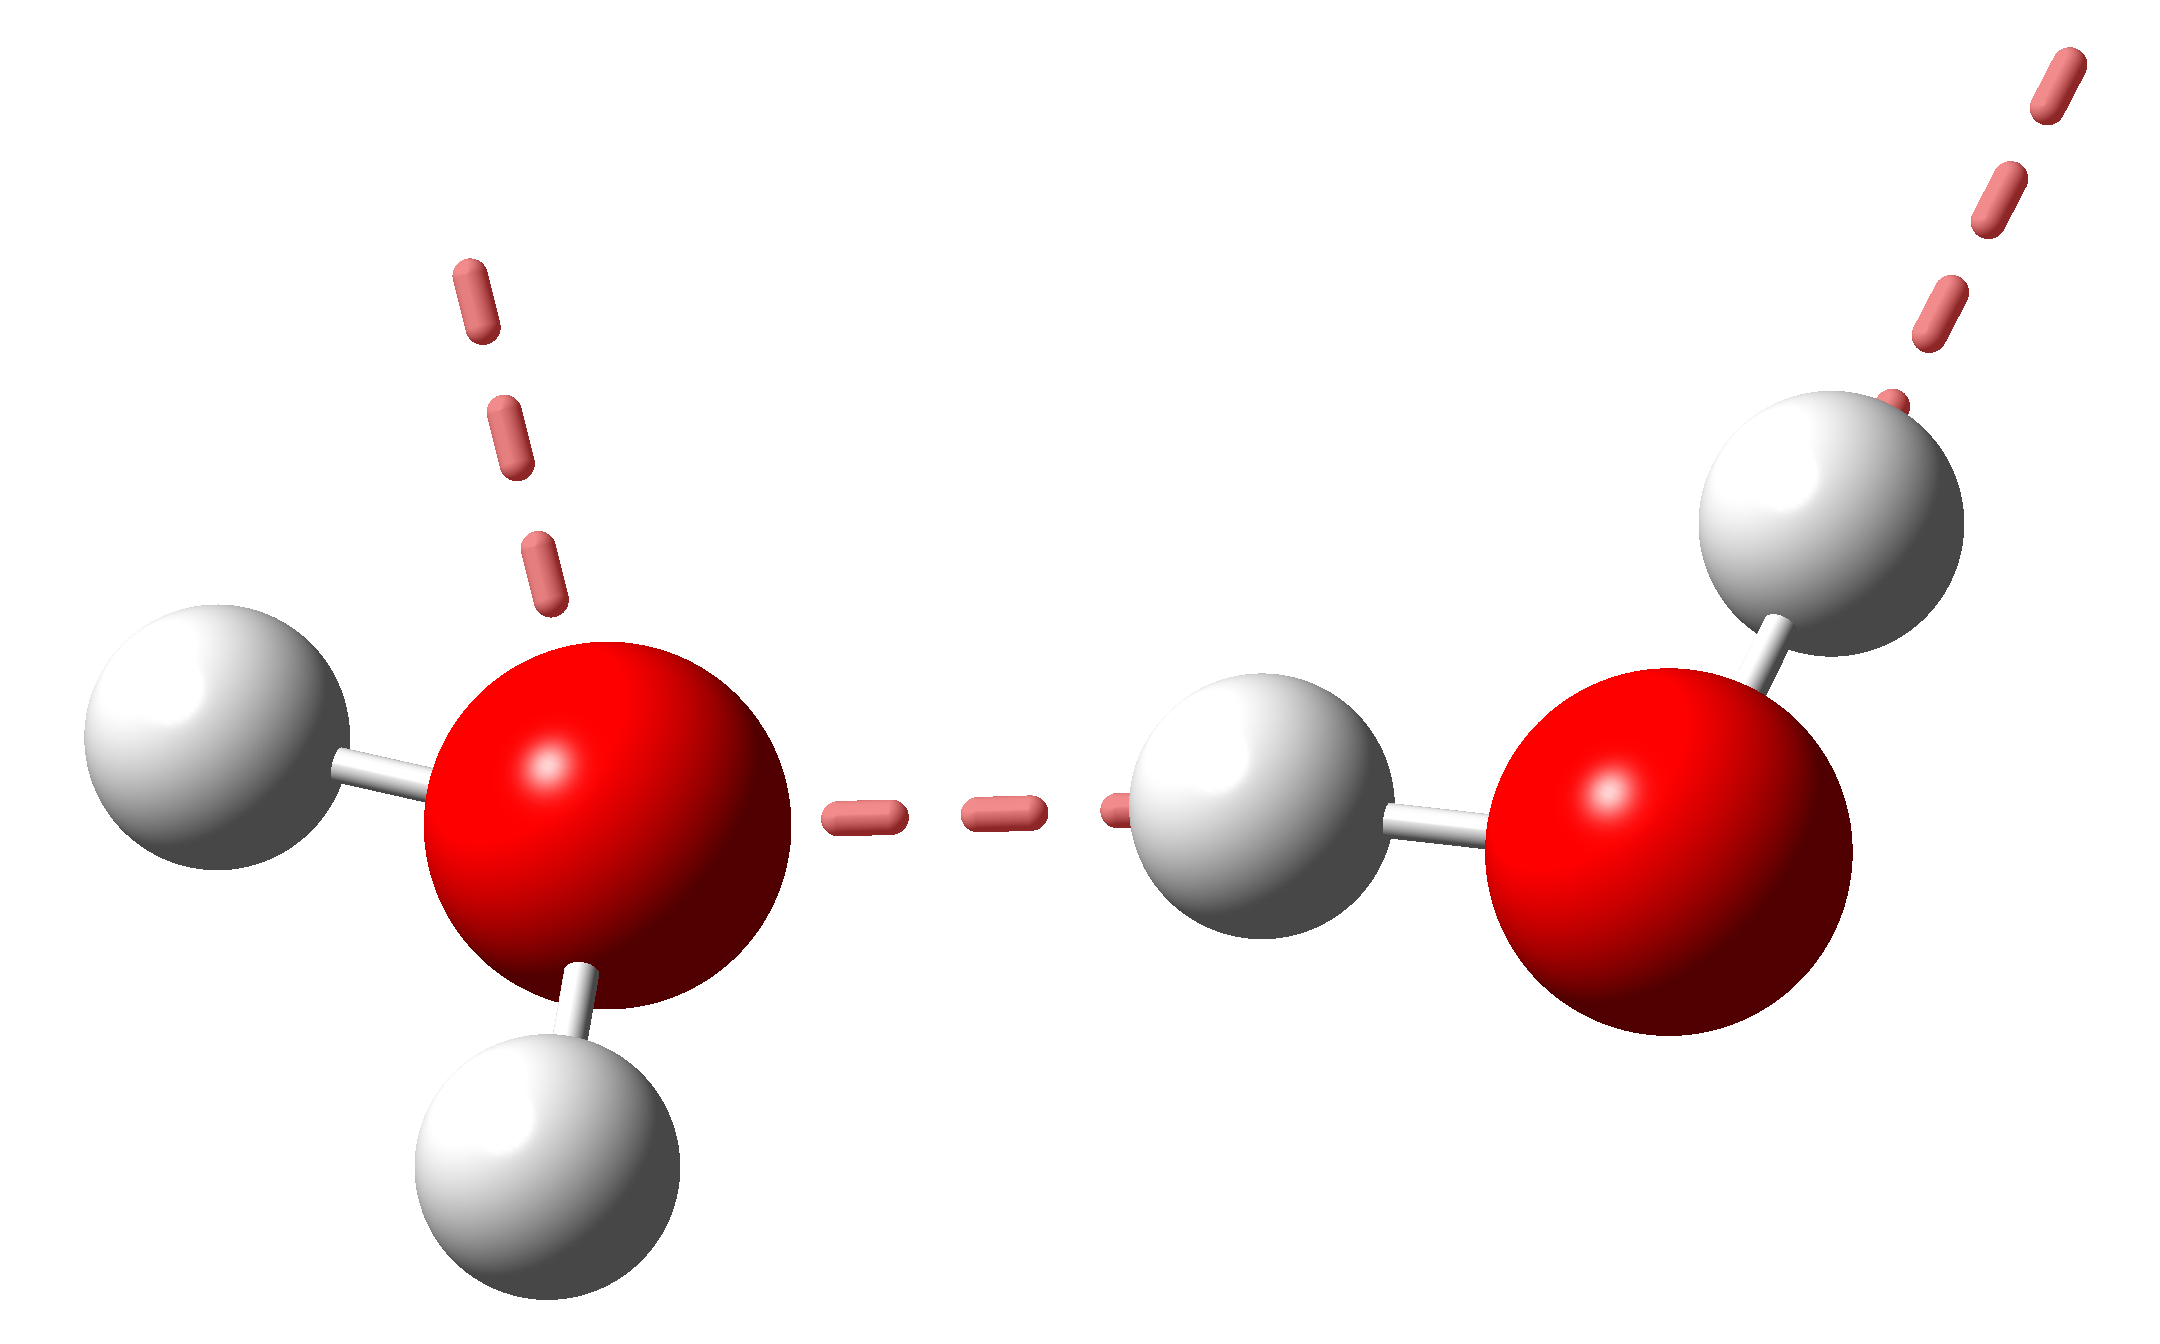
\includegraphics[width=\linewidth]{2/img/dimero_c}
\caption{Anticooperativo}
\label{dimero_c}
\end{subfigure}
\caption{Efectos cooperativos y anticooperativos.}
\label{fig:coop}
\end{figure}

En la Figura \ref{4_h2o} se muestra como 5 moléculas de agua interactúan a
través de EHs, donde la fuerza y direccionalidad de los EHs, así como la
capacidad del agua de interactuar como aceptor y donador al mismo tiempo, hace
a este tipo de sistemas un complejo entramado de interacciones entre las
moléculas de agua, que forman una red tridimensional con una gran variedad de
ángulos y distancias~\cite{liu_science, smith2005}.

Dentro de los principales fenómenos a los que da lugar la gran variedad de
interacciones de EH, dentro de un cúmulo molecular de agua, están los efectos
cooperativos y anticooperativos. Los cuales pueden ser encontrados dentro de
las redes de interacciones experimentadas en los diversos cúmulos, como se
muestra en la Figura \ref{fig:coop}. Para el caso del pentámero \ref{pentamero}
se muestra un cúmulo cíclico homodrómico, es decir, todos las moléculas de agua
están donando y aceptando un EH.  En los casos de las Figuras \ref{dimero_b} y
\ref{dimero_c} se tienen efectos de cooperatividad y de anticooperatividad,
respectivamente; en el caso \ref{dimero_b} se observa como la molécula donadora
de EH está recibiendo dos átomos de hidrógeno, por lo cual es desprovista de
carga, carga que puede ser fácilmente aceptada a través de la donación de un
EH, además de que la molécula aceptora de EH se encuentra donando dos EHs por
lo tal motivo le es muy fácil donar la carga extra con la que cuenta. En
contraste, en la Figura \ref{dimero_c} se puede apreciar como la molécula
donadora de EH también se encuentra como donadora en otro EH por lo que soporta
más carga de lo usual, mientras que, a su vez, la molécula aceptora de EH está
aceptando otro hidrógeno en un segundo EH, por lo que es muy desprovista de
carga.

Estos efectos son mostrados, ejemplificados y descritos en~\citenum{Toche2016},
artículo usado varias veces de referencia y como motivación para esta tesis, de
forma que ésta sirva como una continuación del trabajo anterior, tal como se
expresa en la siguiente sección.

\section{Motivación}

La existencia de enlaces de hidrógeno y como se comportan dentro de sistemas
moleculares ha dado paso a diversos estudios teóricos/computacionales.  Dentro
de estos, se encuentra la publicación realizada por el grupo de investigación
de Tomás Rocha Rinza~\cite{Toche2016}, en donde se propone una jerarquía de los
enlaces de hidrógeno, dentro de cúmulos pequeños de agua.  La clasificación que
se propone en dicho artículo está en función del tipo de coordinación y las
interacciones con primeros vecinos, obteniendo un resultado de seis tipos de
enlaces de hidrógeno, la descripción de estos se muestra en la Tabla
\ref{motivacion}. Estos resultados fueron obtenidos mediante la partición de la
energía electrónica por medio de la metodología IQA, usando geometrías
optimizadas con el método CCSD/aug-cc-pVDZ, y funciones de onda y energías
calculadas con el método MP2/aug-cc-pVTZ.

El trabajo anterior deja en claro una proyección jerárquica de los EH.
Sirviendo éste como motivación, para realizar una continuación a la
tabla, debido a que esta cuenta con la omisión de moléculas de agua
tetracoordinadas.

\chapter{Objetivos}

La presencia de EHs dentro de cúmulos de agua ha planteado diversos problemas,
uno de ellos, es la descripción de las interacciones de EH entre moléculas de
agua en el límite de coordinación. El objetivo principal de esta tesis es el
estudio de las interacciones de las moléculas en el límite de coordinación,
haciendo uso de las herramientas propias de la topología química cuántica. 

Una de las hipótesis principales de este trabajo, es que en el límite de
coordinación, los enlaces de hidrógeno debe empezar a presentar un
comportamiento similar a las interacciones encontradas en el hielo
$\mathrm{I_{h}}$.

Mediante una descomposición de la energía a través del método IQA y del cálculo
de energías electrostáticas utilizando integrales mono- y bielectrónicas, se
pretende abordar los objetivos particulares de esta tesis.

\section{Objetivos Particulares}

\begin{itemize}
\item Reproducir la jerarquía propuesta con anterioridad en~\citenum{Toche2016}
(Tabla \ref{motivacion}), sobre la fortaleza de los EHs en función de la conectividad
de las moléculas de H$_2$O.
\item Extender la clasificación de EHs que se encuentran en cúmulos de agua.
\item Con metodología QTAIM e IQA, buscar efectos cooperativos y
anticooperativos de EH en los diversos cúmulos.
\item Estudiar los efectos a primeros vecinos debidos a la formación de EHs.
\item Analizar las variaciones de la energía clásica y de intercambio-correlación
en función del tipo de EH.
\item Buscar semejanzas entre las interacciones de agua tetracoordinada con
las existentes en el hielo $\mathrm{I_{h}}$.
\end{itemize}

\begin{table}[h]
  \begin{center}
  \caption{Tabla jerárquica presentada en
  (\textit{Phys. Chem. Chem. Phys.}, 2016, \textbf{18}, 19557).}
  \begin{tabular}{c||p{12.5cm}}
Tipo de EH  & Descripción \\ \hline\hline
I           & El átomo de H involucrado en el EH proviene de un doble donador de EH
              y el oxígeno que participa en la interacción actúa como un doble aceptor\\ \hline
II          & ($i$) El H de un doble donador de EH está enlazado con un oxígeno de un aceptor
              sencillo de EH o ($ii$) un oxígeno de un doble aceptor interactúa con un H
              de un donador sencillo \\ \hline
III         & Un enlace de hidrógeno es formado entre dos doble donadores
              de EH o dos dobles aceptores de EH \\ \hline
IV          & Un H de un donador sencillo de EH está enlazado con un oxígeno
              de un aceptor sencillo de EH \\ \hline
V           & ($i$) Un H de un doble aceptor de EH está en contacto con un oxígeno de un
              donador sencillo o ($ii$) el átomo de oxígeno de un doble donador interactúa
              con un hidrógeno de un aceptor sencillo \\ \hline
VI          & El oxígeno de un doble donador de EH interactúa con un H de 
              un doble aceptor de EH \\ 
  \end{tabular}
  \label{motivacion}
  \end{center}
\end{table}

\newpage
\thispagestyle{empty}
